\section{Reflektion}
\begin{frame}
	\frametitle{Refleksion}
	Valg at reflektere over:
	  \begin{itemize}
	    \item{Hime - parser compiler}
	  \end{itemize}
  Uhensigtsmæssige valg:
	  \begin{itemize}
	    \item Alle deklareres skal initialiseres med en værdi - konfliktede med actor
	  \end{itemize}
\end{frame}

\section{Konklusion}
\begin{frame}
	\frametitle{Konklusion}
	Actors som løsning til at beskrive simulationer på en parralel måde
  Fordele:
    \begin{itemize}
      \item Passer godt til vores defintion af en model
      \item Udtrykke funktionalitet som actors
      \item Actors er paralle i natur
      \item Godt til kontinuerlige simulationer
    \end{itemize}
  Ulemper:
    \begin{itemize}
      \item Diskrete simulationer ikke understøttet
    \end{itemize}
\end{frame}

\begin{frame}
	\frametitle{En realisering}
	Actors som erstatninger til funktioner
	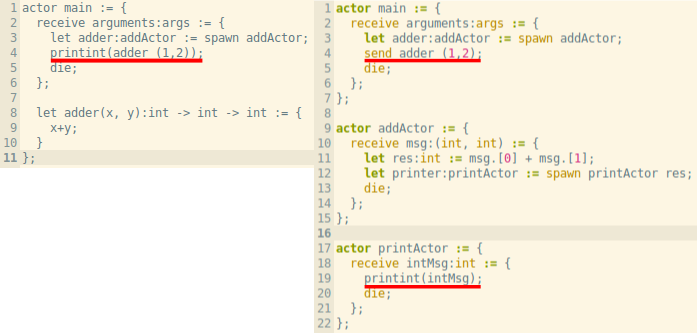
\includegraphics[width=250px]{Images/actorFunc.png}\newline
	Mindre koncist
\end{frame}

\begin{frame}
	\frametitle{Konklusion}
	Actors som løsning til at beskrive simulationer på en parallel måde
  Fordele:
    \begin{itemize}
      \item Passer godt til vores defintion af en model
      \item Udtrykke funktionalitet som actors
      \item Actors er paralle i natur
      \item Godt til kontinuerlige simulationer
    \end{itemize}
  Ulemper:
    \begin{itemize}
      \item Diskrete simulationer ikke understøttet
    \end{itemize}
\end{frame}

\begin{frame}
  \frametitle{Hvorfor er diskrete simulationer ikke understøttet?}
    Arbitrær mængde beskeder sendt under simulering
    
    Vi mangler en metode til at vide hvornår vi er færdige med sende beskeder
\end{end}

\subsection{Environments}
\begin{frame}
	\frametitle{Environments}
	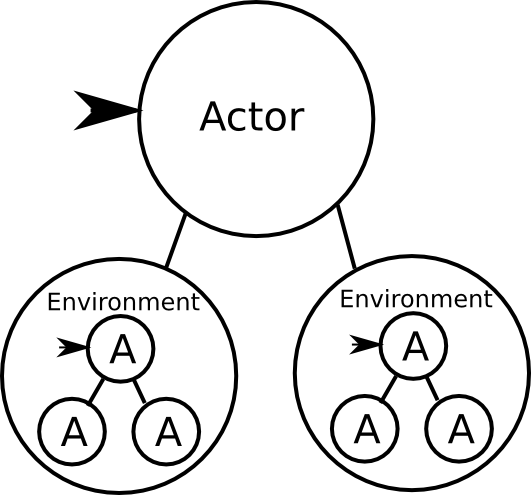
\includegraphics[width=200px]{Images/environment.png}
\end{frame}
\subsection{Iteration steps}
\begin{frame}
  \frametitle{Iteration steps}
  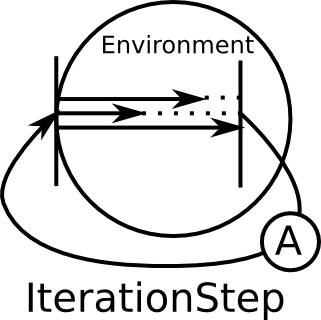
\includegraphics[width=200px]{Images/iteration.png}
\end{frame}

\section{Fremtidigt arbejde}
\begin{frame}
	\frametitle{Fremtidigt arbejde}
	Ideer and konstruktioner ikke inkluderet, endnu: 
  \begin{itemize}
    \item Nedarving(OOP)
    \item Ny konstruktion "reply", programmøren behøver explicit at definere afsender.
    \item Envoriments og iteration steps
  \end{itemize}
\end{frame}
